
% header %{{{1

\documentclass[tikz, border=1mm]{standalone}

\usepackage{amsmath}

\usepackage{tikz}

\usetikzlibrary{calc,angles,quotes,shapes.geometric}

\usepackage{tkz-euclide}

% document %{{{1

% opening %{{{2

\begin{document}
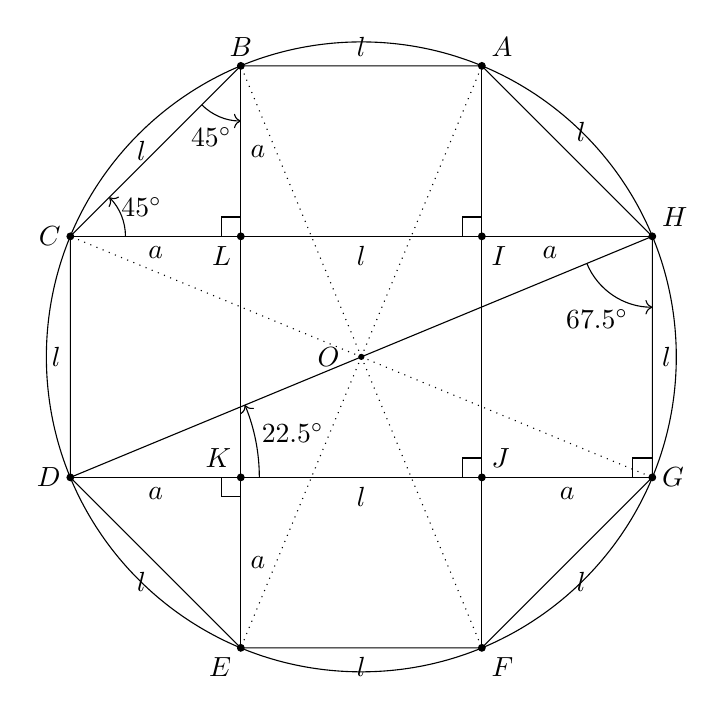
\begin{tikzpicture}[scale=1.0]

% parameters %{{{2

	\def\numsides{8}
	\def\radius{4.0}
	\def\rotation{67.5}

% coordinates %{{{2

	\coordinate (O) at (0,0);

	\foreach \i in {1,...,\numsides} {
		\coordinate (P\i) at ({360/\numsides*(\i-1)+\rotation}:\radius);
	}

% intersections %{{{2

	\tkzInterLL(P1,P6)(P3,P8)\tkzGetPoint{I}
	\tkzInterLL(P1,P6)(P4,P7)\tkzGetPoint{J}
	\tkzInterLL(P2,P5)(P3,P8)\tkzGetPoint{L}
	\tkzInterLL(P2,P5)(P4,P7)\tkzGetPoint{K}

% circle %{{{2

	\draw (O) circle (\radius);

% polygon %{{{2

	\draw (P1) \foreach \i in {2,...,\numsides} { -- (P\i) } -- cycle;

% radiuses %{{{2

	\draw[dotted] (O) -- (P1);
	\draw[dotted] (O) -- (P2);
	\draw[dotted] (O) -- (P3);
	\draw (O) -- (P4);
	\draw[dotted] (O) -- (P5);
	\draw[dotted] (O) -- (P6);
	\draw[dotted] (O) -- (P7);
	\draw (O) -- (P8);

% diagonals %{{{2

	%\draw (P1) -- (P4);
	\draw (P4) -- (P7);
	%\draw (P7) -- (P2);
	\draw (P2) -- (P5);
	%\draw (P5) -- (P8);
	\draw (P8) -- (P3);
	%\draw (P3) -- (P6);
	\draw (P6) -- (P1);

% points, dots, vertices %{{{2

	\foreach \i in {1,...,\numsides} { \fill (P\i) circle (0.5mm); }

	\fill (I) circle (0.5mm);
	\fill (J) circle (0.5mm);
	\fill (K) circle (0.5mm);
	\fill (L) circle (0.5mm);

% points, dots, vertices labels %{{{2

	\node[label={[label distance=0.3mm]left:$O$}] at (O) {};
	\filldraw (O) circle (0.9pt);

	\node[above right] at (P1) {$A$};
	\node[above] at (P2) {$B$};
	\node[left] at (P3) {$C$};
	\node[left] at (P4) {$D$};
	\node[below left] at (P5) {$E$};
	\node[below right] at (P6) {$F$};
	\node[right] at (P7) {$G$};
	\node[above right] at (P8) {$H$};

	\node[below right] at (I) {$I$};
	\node[above right] at (J) {$J$};
	\node[above left] at (K) {$K$};
	\node[below left] at (L) {$L$};

	\node[above] at ($(P1)!0.5!(P2)$) {$l$};
	\node[left] at ($(P2)!0.5!(P3)$) {$l$};
	\node[left] at ($(P3)!0.5!(P4)$) {$l$};
	\node[below left] at ($(P4)!0.5!(P5)$) {$l$};
	\node[below] at ($(P5)!0.5!(P6)$) {$l$};
	\node[below right] at ($(P6)!0.5!(P7)$) {$l$};
	\node[right] at ($(P7)!0.5!(P8)$) {$l$};
	\node[above right] at ($(P8)!0.5!(P1)$) {$l$};

	\node[below] at ($(P3)!0.5!(L)$) {$a$};
	\node[below] at ($(L)!0.5!(I)$) {$l$};
	\node[below] at ($(I)!0.4!(P8)$) {$a$};

	\node[right] at ($(P2)!0.5!(L)$) {$a$};

	\node[below] at ($(P4)!0.5!(K)$) {$a$};
	\node[below] at ($(K)!0.5!(J)$) {$l$};
	\node[below] at ($(J)!0.5!(P7)$) {$a$};

	\node[right] at ($(K)!0.5!(P5)$) {$a$};

% angles labels %{{{2

	\pic[draw, ->, "$45^\circ$", angle radius=0.7cm, angle eccentricity=1.4]
	{angle = P3--P2--L};

	\pic[draw, ->, "$45^\circ$", angle radius=0.7cm, angle eccentricity=1.4]
	{angle = L--P3--P2};

	\pic[draw, ->, "$67.5^\circ$", angle radius=0.9cm, angle eccentricity=1.4]
	{angle = P4--P8--P7};

	\pic[draw, ->, "$22.5^\circ$", angle radius=2.4cm, angle eccentricity=1.2]
	{angle = P7--P4--P8};

% right angle markers %{{{2

	\pic [draw, angle radius=7pt, angle eccentricity=1]
	{right angle = P2--L--P3};

	\pic [draw, angle radius=7pt, angle eccentricity=1]
	{right angle = P4--K--P5};

	\pic [draw, angle radius=7pt, angle eccentricity=1]
	{right angle = P1--I--L};

	\pic [draw, angle radius=7pt, angle eccentricity=1]
	{right angle = P1--J--K};

	\pic [draw, angle radius=7pt, angle eccentricity=1]
	{right angle = P8--P7--J};

% closing %{{{2

\end{tikzpicture}
\end{document}
